\documentclass[titlepage]{article}
\usepackage[bottom=3cm, right=2cm, left=2cm, top=3cm]{geometry}
\usepackage{graphicx}
\usepackage{hyperref}
\usepackage{float}
\restylefloat{table}
\usepackage{amsmath}
\usepackage{booktabs}

\title{SFWRENG 4NL3 Assignment 4: \\ Pretrained Transformers}
\author{Sumanya Gulati}
\date{1 April 2025}

\begin{document}

\begin{titlepage}
    \maketitle
\end{titlepage}

\newpage 

\tableofcontents
\listoftables
\listoffigures

\newpage

\section{Dataset}
For this assignment, I am using the GoEmotions dataset extracted from the HuggingFace can be accessed 
\href{https://huggingface.co/datasets/google-research-datasets/go_emotions}{here}. The task at hand 
involves emotion classification, aiming to identify and categorize the emotions expressed in textual data. This 
is essential for applications such as sentiment analysis, mental health assessment, enhancing human-computer 
interactions and more. \\

The GoEmotions dataset comprises of about 58,000 English Reddit comments, each annotated for 27 distinct emotion 
categories or marked as neutral. The simplified version of the dataset with predefined train, val and test splits 
has been used for this assignment. 

\subsection{Data Collection}
The dataset has been constructed by selecting English-language comments from Reddit by researchers at Amazon Alexa, 
Google Research and Stanford Linguistics. A complete list of authors can be found \href{https://arxiv.org/abs/2005.00547}
{here}. The comments were extracted from Reddit using a variety of automated methods along with data curation techniques 
such as reducing profanity, length filtering, sentiment and emotion balancing, masking and more. Further information 
about the data collection process can be found in section 3.1 of \href{https://arxiv.org/pdf/2005.00547}{this paper}.

\subsection{Dataset Structure}
Each instance of the dataset corresponds to a reddit comment with an ID and one or more emotion annotations including neutral.
The simplified configuration of the dataset which has been used for this assignment, includes:

\begin{itemize}
    \item \texttt{text}: the Reddit comment
    \item \texttt{labels}: the emotional annotations
    \item \texttt{comment\_id}: a unique identifier for the comment
\end{itemize}

The input for the task is a Reddit comment in English and the corresponding output is a set of one or more labels corresponding 
to the 27 emotion categories or neutral, reflecting the emotional content of the comment.

The labels are stored as a list of integers ranging from 0 to 27 where each integer represents an emotion category or neutral. The 
label mapping is as follows:

\begin{table}[H] \label{tab:labels}
    \centering
    \begin{tabular}{lll}
    \toprule
    \textbf{Label Number} & \textbf{Label Category} \\
    \midrule
    0 & admiration \\
    1 & amusement \\
    2 & anger \\
    3 & annoyance \\
    4 & approval \\
    5 & caring \\ 
    6 & confusion \\
    7 & curiosity \\
    8 & desire \\
    9 & disappointment \\
    10 & disapproval \\
    11 & disgust \\
    12 & embarrassment \\
    13 & excitement \\
    14 & fear \\
    15 & gratitude \\
    16 & grief \\
    17 & joy \\
    18 & love \\
    19 & nervousness \\
    20 & optimism \\
    21 & pride \\
    22 & realization \\
    23 & relief \\
    24 & remorse \\
    25 & sadness \\
    26 & surprise \\
    27 & neutral \\
    \bottomrule
    \end{tabular}
    \caption{Label Mapping}
\end{table}

\subsection{Evaluation Metrics}
The following evaluation metrics have been used to assess the performance of the BERT-based model:
\begin{itemize}
    \item Model Performance:
        \begin{itemize}
            \item Emotion-level Precision, Recall, F1: Measured per each emotion in the GoEmotions taxonomy.
            \item Transfer Learning: F1 score on data transferred between domain X and GoEmotions.
        \end{itemize}
    \item Deciison thresholds: No thresholds are used. The data is presented in full granularity.
    \item Uncertainty and variability: Repeated experiments have yielded results with similar taxonomical rankings.
\end{itemize}

The model has been evaluated on 10 publicly available datasets including 9 benchmark datasets presented in compilation 
by \href{https://aclanthology.org/C18-1179/}{Bostan and Klinger} and the \href{https://github.com/google-research/google-research/tree/master/goemotions}
{GoEmotions} eval set. Full details about the evaludation results can be found in the \href{https://arxiv.org/pdf/2005.00547}{paper}.

\subsection{Data Splits}
The dataset is divided into training, validating and test splits as follows:

\begin{table}[H] \label{tab:data_split}
    \centering
    \begin{tabular}{lll}
    \toprule
    \textbf{Data Split} & \textbf{Number of Instances} \\
    \midrule
    Training & 43,410 \\
    Validation & 5,426 \\
    Test & 5,427 \\
    \bottomrule
    \end{tabular}
    \caption{Data Split Overview}
\end{table}

Class distributions for the training and test splits are shown in the figure \ref{fig:class_distribution}.

\begin{figure}[H] \label{fig:class_distribution}
    \centering
    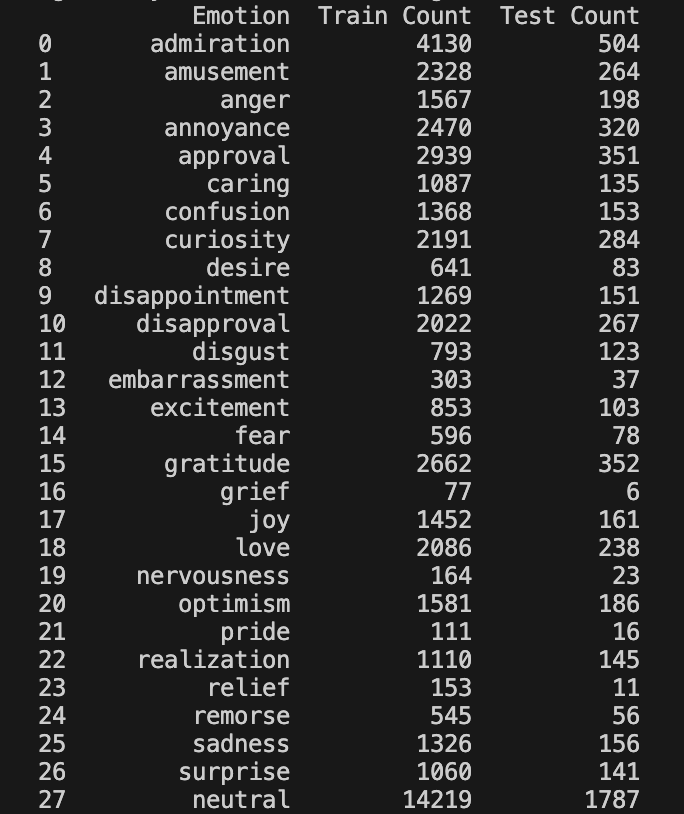
\includegraphics[scale=0.8]{/Users/sg/Desktop/courses/winter-2025/4nl3/assignments/assignment-4/homework4_report/figures/class_distributions.png}
    \caption{Class Distribution in Training and Test Splits}
\end{figure}

\subsection{Additional Features}
Although the comments vary in length, the maximum sequence length has been capped at 30 tokens in the training and evaludation datasets 
to ensure concise and focused emotional expressions. Furthermore, linguistic context consistency has been ensured by only choosing comments 
that are in English.
 
\section{Fine-tuned Models}
For this task, the \href{https://huggingface.co/FacebookAI/roberta-base}{RoBERTa-base} model and the \href{https://huggingface.co/distilbert/distilbert-base-uncased}
{DistilBERT-base-uncased} model have been used. 

\subsection{Model 1: RoBERTa-base}
RoBERTa or "A Robustly Optimized BERT Pretraining Approach" is a transformer-based model that builds on the BERT architecture. It improves upon 
BERT's pretraining methodology by training longer with larger batches over more data, removing the next sentence prediction objective, and dynamically 
changing the masking pattern applied to the training data. The model has approximately 125 million total parameters. 

\subsubsection{Pretraining Dataset}
RoBERTa was pretrained on a diverse and extensive corpus totalling around 160GB of text, including:
\begin{itemize}
    \item BookCorpus which is a dataset of 11,038 unpublished books 
    \item English Wikipedia excluding lists, tables and headers 
    \item CommonCrawl News with over 63 million English news articles from 2016-2019 
    \item OpenWebText which is an open source recreation the WebText dataset used to train GPT-2 
    \item Stories which is a dataset containing a subset of CommonCrawl data filtered to match story-like style of Winograd schemas
\end{itemize}

\subsubsection{Compute Requirements for Pretraining}
The pretraining of RoBERTa-base involved substantial computational resources, including:
\begin{itemize}
    \item \textbf{Hardware}: 1,024 V100 GPUs
    \item \textbf{Training Duration}: 500,000 steps 
    \item \textbf{Batch Size}: 8,000
    \item \textbf{Sequence Length}: 512 tokens
    \item \textbf{Optimizer}: Adam with a learning rate of 6e-4 
\end{itemize}

\subsection{Model 2: DistilBERT-base-uncased}
DistilBERT is a distilled version of BERT, designed to be smaller, faster, and more efficient while retaining 97\% of BERT's language 
understanding capabilities. It achieves this through knowledge distillation during the pretraining phase, effectively reducing the model 
size by 40\%. The model has approximately 66 million total parameters.

\subsubsection{Pretraining Dataset}
DistilBERT was pretrained on the same corpus as BERT, which includes:
\begin{itemize}
    \item BookCorpus which is a dataset of 11,038 unpublished books
    \item English Wikipedia excluding lists, tables and headers
\end{itemize}

\subsubsection{Compute Requirements for Pretraining}
The pretraining of DistilBERT-base-uncased utilized:
\begin{itemize}
    \item \textbf{Hardware}: 8 16GB V100 GPUs
    \item \textbf{Training Duration}: 90 hours
\end{itemize}

\subsection{Fine-Tuning Steps}
The RoBERT-a and DistilBERT-base-uncased models were fine-tuned on the GoEmotions dataset using the following process:
\begin{enumerate}
    \item Dataset Preparation
        \begin{itemize}
            \item Loaded the GoEmotions dataset with simplified labels (27 categories in total).
            \item Verified the dataset structure and label distribution.
            \item Used the predefined train, validation and test splits.
        \end{itemize}
    \item Preprocessing 
        \begin{itemize}
            \item Tokenize the data using RoBERTa's byte-level Byte-Pair Encoding (BPE) tokenizer and DistilBERT's WordPiece tokenizer.
            \item Applied truncation and padding to a maximum sequence length of 128 tokens.
            \item Converted datasets to PyTorch format.
        \end{itemize}
    \item Hyperparameter Optimization
        \begin{itemize}
            \item Optimized for weighted F1 score on the validation set.
            \item Tuned parameters such as learning rate, weight decay and batch size.
            \item Performed 5 trials per model to balance optimization quality with computational time.
        \end{itemize}
    \item Model Configuration 
        \begin{itemize}
            \item Configured both models with a classification head for 27 labels.
            \item Implemented early stopping with a patience of 3 epochs.
            \item Used mixed precision training for memory efficiency.
            \item Applied gradient accumulation (steps=2) to stimulate larger batch sizes.
        \end{itemize}
    \item Fine-tuning Process 
        \begin{itemize}
            \item Trained both models using the Trainer API from HuggingFace Transformers.
            \item Applied the best hyperparameters found during optimization.
            \item Trained for up to 5 epochs with early stopping.
            \item Envaluated performance after each epoch on the validation set.
            \item Saved the best checkpoint based on validation performance.
        \end{itemize}
\end{enumerate}

\end{document}